
\chapter{Specifications}
The hardware and software used in this project was chosen to be as close as possible to the 
hardware used by Argus in their underwater vehicles. This gives us 
a scenario closer to the real hardware, and imposes the same 
restrictions on us as would be imposed in real world applications.

\section{Hardware}

\subsection{Argus hardware}
The hardware used by Argus is only mentioned as 
\begin{quote}
$1\times$ Foc/Zoom camera \\
Optional HDTV Camera 1080i \\
$1\times$ Lowlight Black \& White camera \\
\end{quote}
in \citet{argusROV}. After some mailing with Argus, they provided us 
with the specific details of this HD Camera, which is what we are interested in. 
The most interesting parts of the camera specification is shown in table \vref{tbl:fcbh11}.

\subsection{High definition video hardware}
The camera used by Argus is the Sony FCB-H11 \citet{fcbh11}. 

\begin{table}[htbp]
	\centering
	\begin{tabular}{ll}
	
		\toprule
			Camera specification 	& Detail \\
		\midrule
			Image sensor 			& 1/3-type CMOS \\
			Pixels 					& $\approx2\times10^{6}$ Pixels \\
			Zoom 					& $12\times$ (Digital) and $10\times$ (Optical) \\
			Gain 					& Auto and manual (\SI{-3}{\deci\bel} to \SI{18}{\deci\bel}) \\
			S/N						& > 50dB \\
			Minimum illumination 	& \SI{1.2}{\lux} (F1.8 50IRE) \\
									& \SI{1.0}{\lux} (ICR ON F1.8 50IRE) \\
			Video output			& HD Analog component Y/Pb/Pr \\
									& HD Digital LVDS Y/Pb/Pr 8 bit \\
									& SD VBS \SI{1.0}{\volt_{p-p}} Negative sync Y/C \\
			Camera control interface& VISCA TTL \\
			Operating temperature	& \SI{0}{\celsius} to \SI{45}{\celsius} \\
			Power consumption		& \SI{9}{\volt} $\pm$ \SI{3}{\volt} DC, \SI{4.8}{\watt} \\
		\bottomrule
	\end{tabular}
	\caption{Selected FCB-H11 Specifications}
	\label{tbl:fcbh11}
\end{table}


As seen in \vref{tbl:fcbh11}, the camera outputs HD Digital LVDS\footnote{Low-Voltage Differential Signal} signals.
Due to the open standard used by this camera, there are quite a few different add-on cards that 
converts this LVDS signal to other, more robust signals for different applications.

\subsubsection{VISCA camera control}\label{sec:visca}
The FCB-H11 can be controlled by the open Sony VISCA protocol. This is based of RS-232C at TTL signal levels
at 9600 bauds. Newer cameras can support RS-232C at up to 38400 bauds using the 8N1 configuration and no flow control. 
VISCA contains a rich set of commands to control professional video systems. It even is compatible with 
the broadcast networking specification of the RS-232C which means that a single signal line can contain 
8 devices including the PC, as it uses \SI{1}{\byte} for addressing.

The implementation of the VISCA protocol that is supported by the FCB-H11 is given in \citet{fcbh11tech}. 
The FCB-H11 does for instance not implement the broadcasting function of VISCA, and must therefore 
be on a single RS-232C signal line. 

In addition to normal power on/off and setup data, the VISCA protocol can send a slew of different 
control messages. Amongst these are zoom, focus, white balancing, spot focus and different video effects as 
black and white or negative images that is being processed by the image processor on the camera. This 
makes the camera very versatile, either by direct control from a PC using a TTL level translator or 
by any micro controller using USART.

Sony provides a basic program for implementing VISCA. In addition to this, a open source C library for Windows, Linux and 
AVR is available at \url{http://sourceforge.net/projects/libvisca/}. This makes it very easy to 
integrate VISCA into the software if needed.

\begin{figure}[htbp]
	\centering
	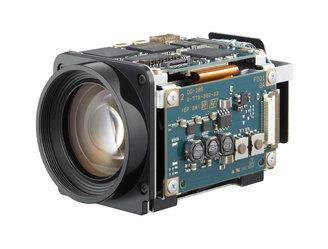
\includegraphics{fcbh11}
	\caption{Sony FCB-H11 High Definition Block Camera}
	\label{fig:fcb-h11}
\end{figure}

\subsection{High definition video signalling}



Many different interface boards are available for the FCB-H11 which gives different output formats from the camera and 
provides different control interfaces to the camera..
The most normal interface cards provides HDMI, USB, Ethernet, SDI and HD-SDI outputs in 
different configurations and combinations. A comparison of the different technologies is shown in \vref{tbl:transmission_systems}.

\begin{table}[htbp]
	\centering
	\begin{tabular}{llllr}
		\toprule
			System 				& Bitrate 							& Distance 						& Protocol 	& Compression Ratio \\
		\midrule
			HDMI 				& \SI{10.2}{\giga bit\per\second}	& $\approx$ \SI{15}{\metre}		& TMDS 		& 0\% \\
			USB 3.0 			& \SI{5}{\giga bit\per\second}		& $\approx$ \SI{5}{\metre}		& Serial	& 0\% \\
			Gigabit Ethernet	& \SI{1}{\giga bit\per\second}		& $\approx$ \SI{220}{\metre}	& Serial	& $\approx$ 30\% \\
			SDI					& \SI{360}{\mega bit\per\second}	& $\approx$ \SI{300}{\metre}	& NRZI 		& $\approx$ 75\% \\
			HD-SDI				& \SI{1.485}{\giga bit\per\second}	& $\approx$ \SI{300}{\metre}	& NRZI		& 0\% \\
		\bottomrule
	\end{tabular}
	\caption{Different signalling systems}
	\label{tbl:transmission_systems}
\end{table}


For this project, it was decided that we should 
try to get a interface that did have more capacity than the camera produces. Looking 
at the different options in \vref{tbl:transmission_systems}, and also thinking of the transmission length, HD-SDI
was chosen as the desired technology for transferring the video stream from the camera.

\subsubsection{HD-SDI}\label{sec:hdsdi}
The HD-SDI signalling standard is a improvement to the older SDI standard. Where the SDI can only transfer images
in maximum 576i format, the HD-SDI standard i capable of transferring 720p and 1080i video. Newer versions 
of the HD-SDI standard is also capable of 1080p and 4K video streams. 

HD-SDI is a professional video standard mainly used by TV stations and in other high end systems. It is 
defined and maintained by the Society of Motion Picture \& Television Engineers, SMPTE. More information 
on the SDI family can be found on the SMPTE website at \url{https://www.smpte.org/standards/}.

Some of the niceties of the HD-SDI interface, in addition to the bandwidth and transmission length, is 
that the interface is self-clocked, self-correcting and supports self setup. This means that the 
interface is more or less plug-and-play\footnote{Bad vibes ohoy}. 

\begin{figure}[htbp]
	\centering
	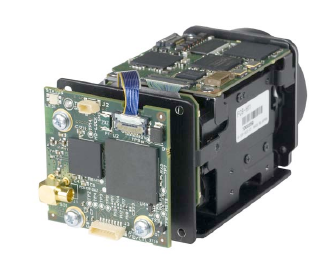
\includegraphics[width=0.8\linewidth]{em15710}
	\caption{Intertest EM15710 iShoot-FCB-HDSDI interface}
	\label{fig:em15710}
\end{figure}

\subsubsection{Gigabit Ethernet}
During the last month of the project, two Gigabit Ethernet modules were acquired. The modules is primarily 
going to be used in future projects, as cabling and instrumentation over ethernet turns out to be simpler. 

The interface is shown in figure \vref{fig:iport} with the FCB-H11 connected. This unit gives access to the VISCA protocol described 
in \vref{sec:visca} over ethernet, together with the video feed. This means that the feed and control signals can be superimposed 
on any ethernet compatible infrastructure, which is both cheaper and more readily available, as well as easier 
to interface with most computers today.

\begin{figure}[htbp]
	\centering
	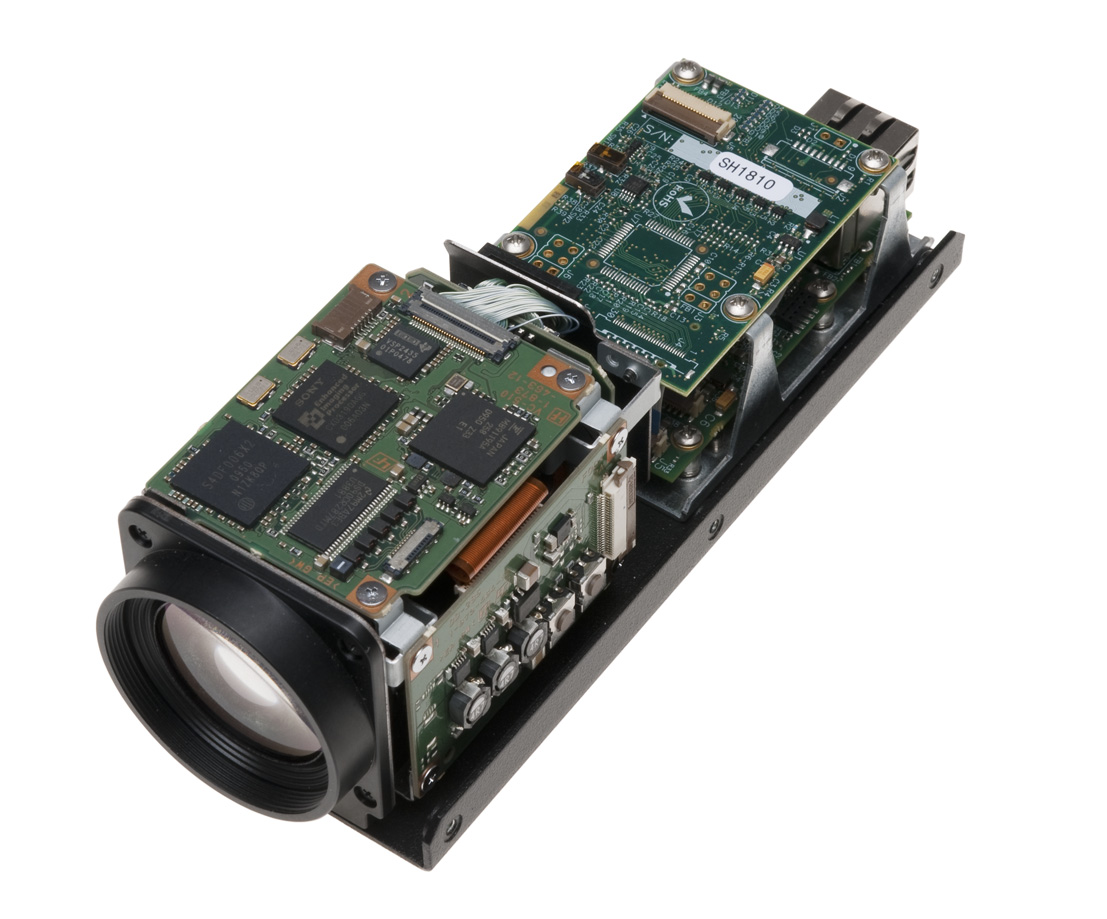
\includegraphics[width=0.8\linewidth]{iport}
	\caption{Pleora SB-Pro IP Engine for Sony FCB-H11}
	\label{fig:iport}
\end{figure}

\subsubsection{Video stream grabbing}
The capture of video streams from a HD-SDI interface usually needs specifically designed hardware that 
connects to one of the internal buses in the computer to get high enough bandwidth. This is usually 
done using a PCI Express card that can support multiple HD-SDI streams simultaneously. 

This is however not practical, as we are going to use different computers and laptops during our testing. 
It would therefore be better to get a external capture interface that connects to the computers using a 
external computer interface. Thankfully, with the development of USB 3.0 we are able 
to support the bandwidth requirements for HD signal.

The Ultrastudio SDI from Blackmagic Design was chosen as the stream grabber. This is a industry standard 
supplier that recently developed this external capture unit. More information on this can be found at 
\url{http://www.blackmagicdesign.com/products/ultrastudiousb3/} and the unit is shown in \vref{fig:ultrastudio_sdi}.

\begin{figure}[htbp]
	\centering
	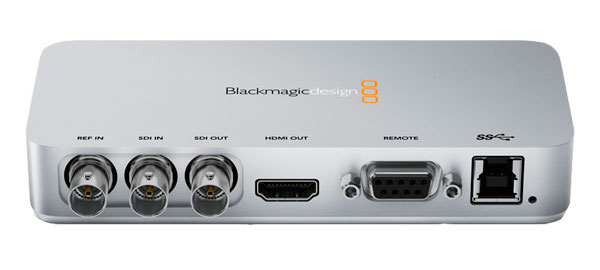
\includegraphics[width=0.8\linewidth]{ultrastudiosdi}
	\caption{Blackmagic Ultrastudio SDI for USB 3.0}
	\label{fig:ultrastudio_sdi}
\end{figure}

The Ultrastudio SDI unit gives HD-SDI in together with HD-SDI out, HDMI out and USB 3.0. The 
extra HDMI out makes it easy to connect a external monitor while capturing to get better visual feedback.



\section{Software}
The software used is split into two different categories; the video capture software provided by Blackmagic 
Design, and the video analysis software developed in this project. Fortunately, the Ultrastudio 
unit comes with WDM\footnote{Windows Device Management} drivers and DSHOW\footnote{Direct Show, part of DirectX} 
filters, and a software development kit which makes it somewhat easy to connect to the unit and stream 
the video from it in real time. 


\subsection{High definition video capture}

\subsection{High definition video analysis}

\subsection{Real time constraints}

